%Comparison.tex
\section{Lightcurve Comparison}

From these magnitude vs. time plots, we can calculate a linear fit to the climb between cooling trough and plateau. This provides a quick comparison for how quickly the brightness rises to the plateau in the first moments of the supernovae.

Below are plots of the U band of 1987A and 2014J with a linear fit. The U band has been selected because in both lightcurves, its rise is very linear and free of the "shoulder" observed in the 2014J spectrum. For both supernovae, a range has been selected to focus only on the specific, initial climb. For 1987A, this is 47400 through 47800 seconds. For 2014J, this is 56700 through 56720 seconds.

\begin{figure}[h]
	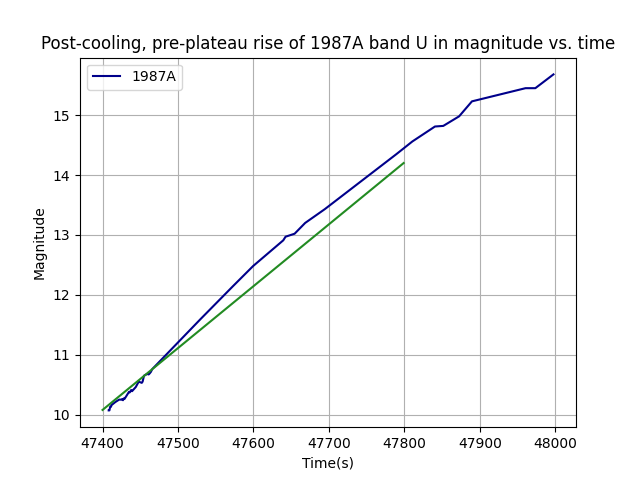
\includegraphics[width=1.0\textwidth]{1987A_U_linear.png}
	\caption{Linear fit to magnitude vs. time in U band of 1987A. Slope for 1987A = 0.0103319.}
\end{figure}

\begin{figure}[h]
	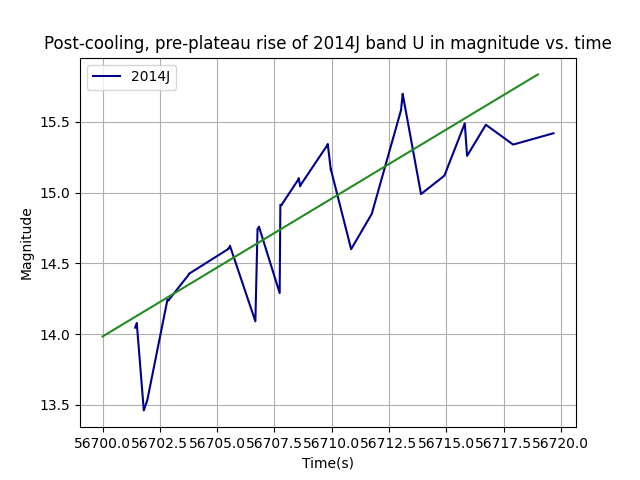
\includegraphics[width=1.0\textwidth]{2014J_U_linear.png}
	\caption{Linear fit to magnitude vs. time in U band of 1987A. Slope for 2014J = 0.0975568.}
\end{figure}

From these plots, we observe a slope of 0.0103319 for the U band of 1987A and a slope of 0.0975568 for the U band of 2014J. This difference fits our expectations based on the typical lightcurves of Type IIP and Type Ia supernovae: Type Ia tend to rise in brightness much more sharply at the start, while Type IIP climb more slowly. 1987A and 2014J are typical examples of this feature.

